\begin{center}
\emph{PRISMA (Prima Rete Italiana per la Sorveglianza sistematica di Meteore e
Atmosfera)\footnote{Da qui in avanti ci si riferirà ad essa solo con la sigla corrispondente.} è un progetto collaborativo proposto e coordinato dall’Istituto Nazionale
di Astrofisica (INAF) a cui partecipano Istituti di ricerca, associazioni, scuole.
L’elenco completo dei partecipanti è disponibile sul sito www.prisma.inaf.it}
\end{center}

\section{Il Progetto}
\begin{wrapfigure}{l}{0.3\textwidth}
    \vspace{-30pt}
    \begin{center}
    
\includegraphics[width=0.3\textwidth]{images/logo.png}
    \end{center}
    \vspace{-22pt}
\end{wrapfigure}

Il progetto PRISMA prevede la realizzazione di una rete italiana di camere all-sky per l'osservazione di meteore brillanti (fireball e bolidi), al fine di determinare le orbite degli oggetti che le provocano e delimitare con un buon grado di approssimazione le aree dell'eventuale caduta di frammenti per poter recuperare le meteoriti.

Il monitoraggio sistematico della copertura nuvolosa e dell'attività elettrica sarà usato per la validazione di modelli meteorologici. I dati raccolti in maniera sistematica contribuiranno al perfezionamento dei modelli di interazione dei corpi cosmici con l'atmosfera che a tutt'oggi presentano ancora molte lacune a causa della mancanza di dati osservativi di qualità.
\cite{progetto-PRISMA}


\section{Fireball e Bolide}
Fireball e bolide sono termini astronomici per indicare meteore particolarmente brillanti e spettacolari che possono essere agevolmente viste anche di giorno da un'ampia regione. 

Per meteoroide si intende un frammento di asteroide o cometa in orbita attorno al Sole che ha una dimensione inferiore al metro. Le meteore, anche chiamate stelle cadenti, sono la traccia visibile dei meteoroidi che entrano nell'atmosfera terrestre con un'alta velocità. 

Un fireball è una meteora che raggiunge una luminosità uguale o superiore a quella di Venere, il terzo astro più brillante nel cielo. I fireball che esplodono e si frammentano durante la caduta sono chiamati in gergo tecnico bolidi, anche se i due termini sono spesso utilizzati indifferentemente. Durante la fase di ingresso in atmosfera, l'oggetto impattante è rallentato e riscaldato per attrito. Nella parte frontale il gas atmosferico è compresso e scaldato e forma una zona di shock. Parte dell'energia generata dall'attrito provoca l'erosione dell'oggetto, e nella maggior parte dei casi la sua successiva rottura. La frammentazione aumenta l'effetto dell'attrito, causando ulteriore erosione e frammentazione, fino a quando la differenza tra le forze di pressione di fronte e dietro l'oggetto ne provocano la completa e catastrofica distruzione. Sebbene in genere gli oggetti che generano un fireball non siano grandi a sufficienza per sopravvivere intatti al passaggio in atmosfera, spesso frammenti o meteoriti possono venir recuperati a terra.
\cite{bolide-fireball}

\section{Enti Coinvolti}
Al progetto partecipano ricercatori dell'Istituto Nazionale di Astrofisica e delle Università, Gruppi Astrofili e Osservatori Astronomici e Meteorologici regionali e locali. Anche le Scuole sono coinvolte con un programma didattico e con laboratori di astronomia che intendono far partecipare gli studenti e i singoli cittadini alle attività di ricerca del progetto, fianco a fianco con i ricercatori. Questo aspetto del progetto si situa nell'ambito di PRISMA-Edu, che viene sviluppato grazie anche al sostegno finanziario delle fondazioni bancarie. \cite{progetto-PRISMA}

Per quanto riguarda il lato informatico del progetto, PRISMA si appoggia all'azienda esterna N3 Srl \cite{n3srl}. Il progetto illustrato nei successivi capitoli è avvenuto in collaborazione con questa azienda.

\begin{figure}[b]

\begin{subfigure}{\textwidth}
\begin{center}
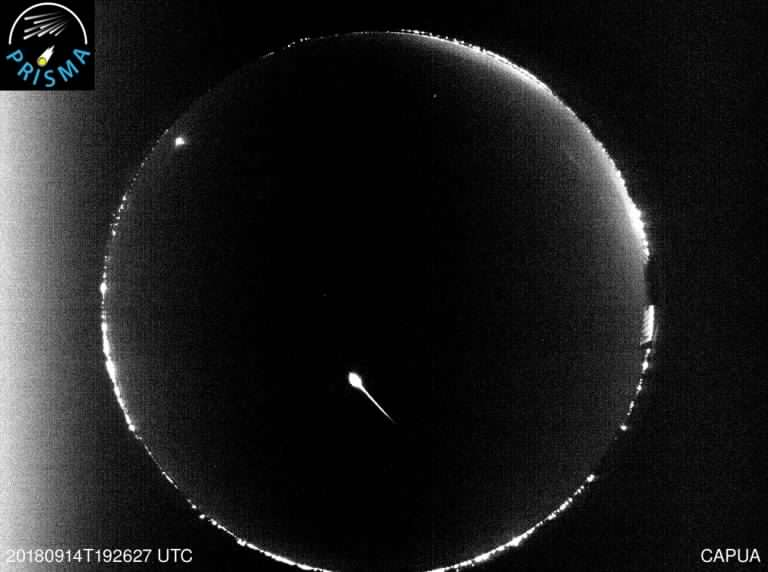
\includegraphics[width=0.9\textwidth]{images/CAPUA_20180914.jpg}
\caption{Rilevazione del 14/09/18 19:26:08 UTC}
\end{center}
\end{subfigure}

\vspace{12pt}

\begin{subfigure}{\textwidth}
\begin{center}
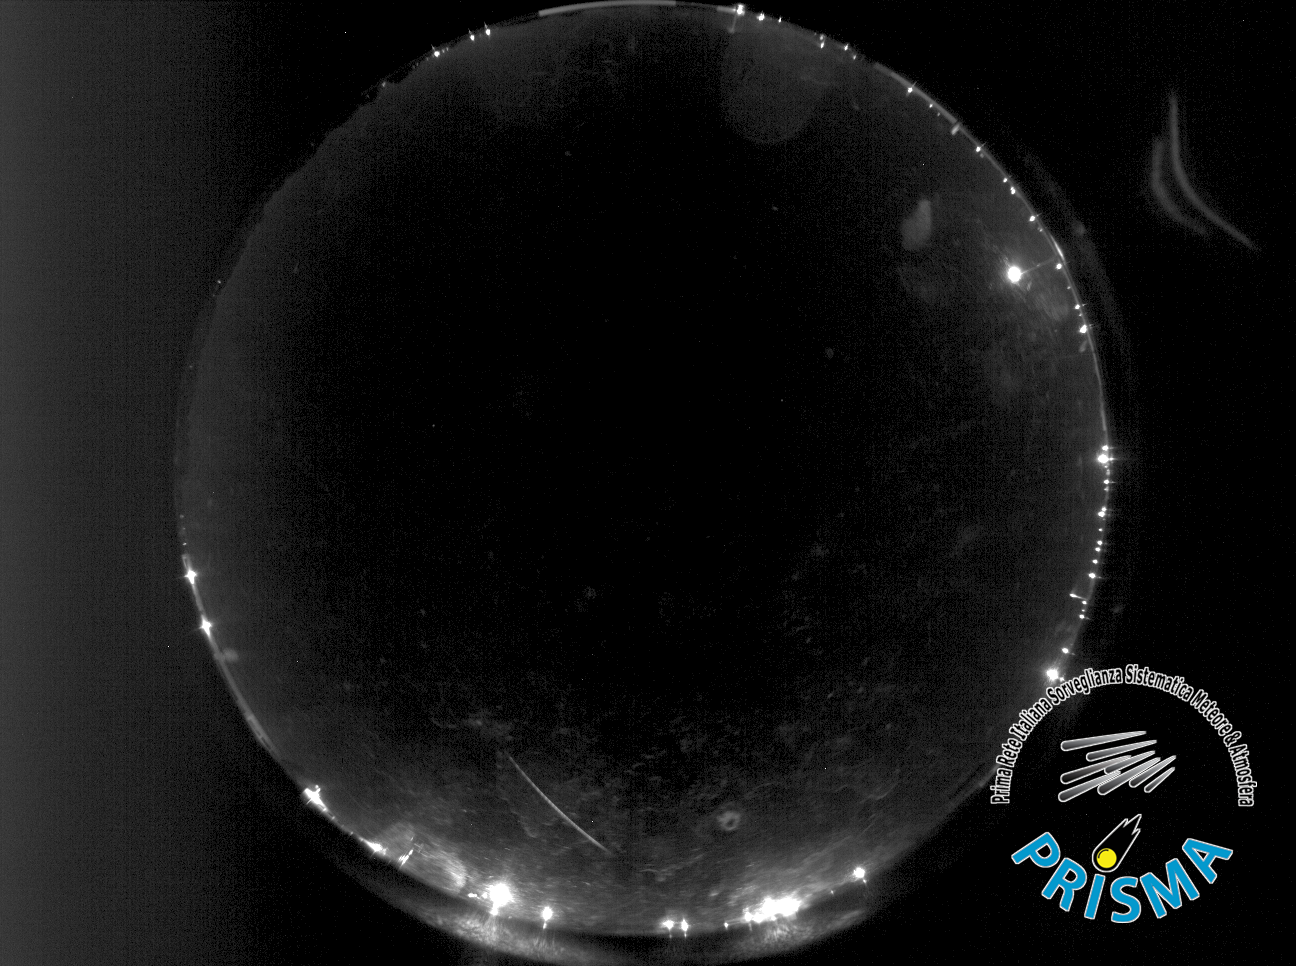
\includegraphics[width=0.9\textwidth]{images/CODOGNO_22062022.png}
\caption{Rilevazione del 22/06/22 00:12:00 UTC}
\label{fig:codogno-2206}
\end{center}
\end{subfigure}

\caption{Rilevazioni di meteore ad opera di PRISMA}
\end{figure}